\chapter{Chapter-3 Methodology}

\section{Data Preparation}

The dataset used in this study consists of images categorized into four classes: Closed, Open, No Yawn, and Yawn. The images are preprocessed and transformed using \texttt{torchvision.transforms} to ensure consistency and improve model performance. Data augmentation techniques, such as resizing, cropping, and normalization, are applied to enhance the dataset's diversity.

\section{WorkFlow}

This section describes the overall workflow of the methodology, including data preprocessing, model training, and evaluation steps.

\begin{figure}[H]
  \centering
  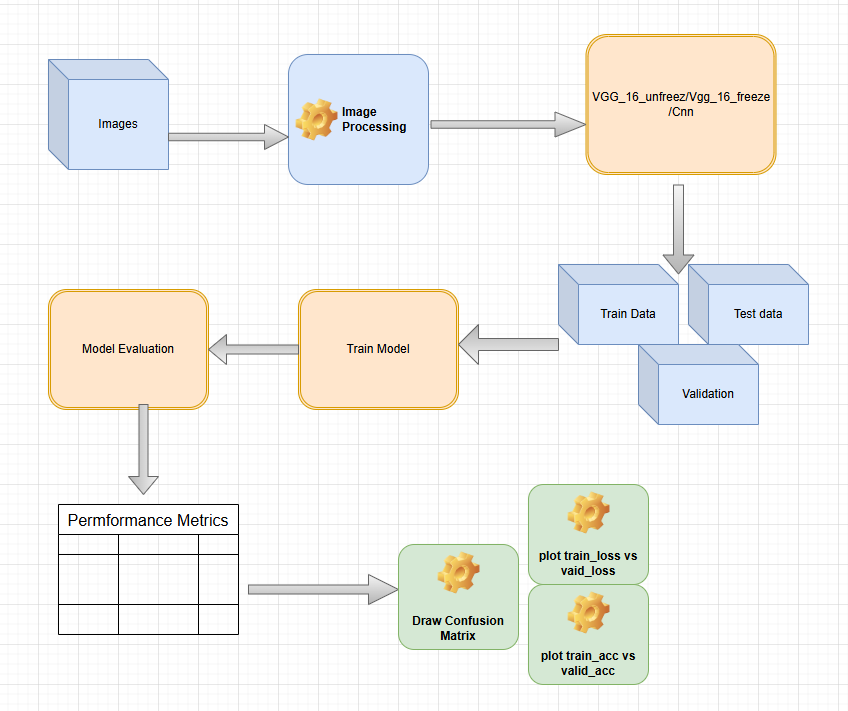
\includegraphics[width=1\linewidth]{common_workflow.png}
  \caption{Workflow Step}
  \label{fig:workflow1}
\end{figure}

\subsection{Step 1: Data Collection}

The first step involves collecting the dataset, which consists of images categorized into four classes: Closed, Open, No Yawn, and Yawn. This dataset is crucial for training and evaluating the models.

\subsection{Step 2: Data Preprocessing}

In this step, the collected images are preprocessed to ensure consistency and improve model performance. Preprocessing includes resizing, cropping, and normalization using \texttt{torchvision.transforms}. Data augmentation techniques are also applied to enhance the dataset's diversity.

\subsection{Step 3: Model Training}

The preprocessed data is then used to train the models. Various model architectures, such as VGG-16 with Batch Normalization, VGG-16 with Unfreezing and Learning Rate Scheduler, and a Lightweight CNN, are employed. Each model is fine-tuned and optimized for the task.

\subsection{Step 4: Model Evaluation}

After training, the models are evaluated using validation data. The performance metrics, such as accuracy and loss, are tracked and analyzed to determine the effectiveness of each model.


\section{Model Architectures}

\subsection{Model 1: VGG-16 with Batch Normalization}

The first model is based on the VGG-16 architecture with batch normalization. The model is pre-trained on ImageNet and fine-tuned for the DDD task. The last three convolutional layers are unfrozen to allow fine-tuning.

\begin{verbatim}
vgg16 = models.vgg16_bn(weights=models.VGG16_BN_Weights.DEFAULT)  # Use pretrained weights

# Freeze training for all layers in the feature extractor
for param in vgg16.features.parameters():
    param.requires_grad = False

# Unfreeze the last three convolutional layers
conv_layers_to_unfreeze = []
for i in range(len(vgg16.features) - 1, -1, -1):  # Traverse in reverse
    if isinstance(vgg16.features[i], nn.Conv2d):
        conv_layers_to_unfreeze.append(i)
    if len(conv_layers_to_unfreeze) == 3:
        break

# Unfreeze these layers
for i in conv_layers_to_unfreeze:
    for param in vgg16.features[i].parameters():
        param.requires_grad = True

# Modify the classifier to adapt to the number of classes
num_features = vgg16.classifier[6].in_features  # Get input features of the last layer
features = list(vgg16.classifier.children())[:-1]  # Remove last layer
features.append(nn.Linear(num_features, 4))  # Add a new layer for 4 classes
vgg16.classifier = nn.Sequential(*features)  # Replace the classifier
vgg16 = vgg16.to(device)
\end{verbatim}

\subsection{Model 2: VGG-16 with Unfreezing and Learning Rate Scheduler}

The second model is similar to the first but includes a learning rate scheduler to adjust the learning rate based on the validation loss.

\begin{verbatim}
criterion = nn.CrossEntropyLoss()
optimizer = optim.Adam(vgg16.parameters(), lr=0.0001, weight_decay=0.01)
exp_lr_scheduler = lr_scheduler.ReduceLROnPlateau(optimizer, mode='min', factor=0.5, patience=3)
\end{verbatim}

\subsection{Model 3: Lightweight CNN}

The third model is a lightweight CNN designed from scratch to balance computational efficiency and accuracy.

\begin{verbatim}
class LightWeightCNN(nn.Module):
    def __init__(self):
        super(LightWeightCNN, self).__init__()
        self.conv1 = nn.Conv2d(in_channels=3, out_channels=32, kernel_size=3, stride=1, padding=1)
        self.conv2 = nn.Conv2d(in_channels=32, out_channels=64, kernel_size=3, stride=1, padding=1)
        self.conv3 = nn.Conv2d(in_channels=64, out_channels=128, kernel_size=3, stride=1, padding=1)
        self.conv4 = nn.Conv2d(in_channels=128, out_channels=128, kernel_size=3, stride=1, padding=1)
        self.conv5 = nn.Conv2d(in_channels=128, out_channels=128, kernel_size=3, stride=1, padding=1)
        self.pool = nn.MaxPool2d(kernel_size=2, stride=2)
        self.fc1 = nn.Linear(in_features=128*7*7, out_features=1024)
        self.fc2 = nn.Linear(in_features=1024, out_features=4)
        self.dropout = nn.Dropout2d(0.2)
        self.dropout1 = nn.Dropout(0.2)

    def forward(self, x):
        x = self.dropout(self.pool(F.relu(self.conv1(x))))
        x = self.dropout(self.pool(F.relu(self.conv2(x))))
        x = self.dropout(self.pool(F.relu(self.conv3(x))))
        x = self.pool(F.relu(self.conv4(x)))
        x = self.pool(F.relu(self.conv5(x)))
        x = x.view(-1, 128*7*7)
        x = self.dropout1(x)
        x = F.relu(self.fc1(x))
        x = self.dropout1(x)
        x = self.fc2(x)
        return x
\end{verbatim}

\section{Training}

The models are trained using the following parameters:

\begin{itemize}
    \item \textbf{Optimizer:} SGD with learning rate 0.01 for the lightweight CNN, and Adam with learning rate 0.0001 for the VGG-16 models.
    \item \textbf{Loss Function:} CrossEntropyLoss
    \item \textbf{Epochs:} 50
\end{itemize}

Training and validation losses and accuracies are tracked and printed for each epoch. The models are saved if the validation loss decreases.